\section{Introduction}

    \subparagraph{}Le but de ce {\color{info}deuxième travail} est d'implémenter un circuit contenant au moins une source de tension ainsi qu'une source de courant avec 
    plusieurs résistances. Il s'agira ensuite de calculer les tensions en utilisant la méthode des noeuds et enfin de simuler le circuit avec le logiciel \textit{LTspice}
    afin de démontrer l'exactitude des calculs.\\[1.5cm]
    
    \begin{titletbox}{À l'attention du correcteur / correctrice}{warning}
        N'hésitez pas à zoomer sur les schémas du circuit et autres images afin d'y voir plus clair.
    \end{titletbox}

\section{Schéma initial du circuit}

    \begin{figure}[H]
        \centering
        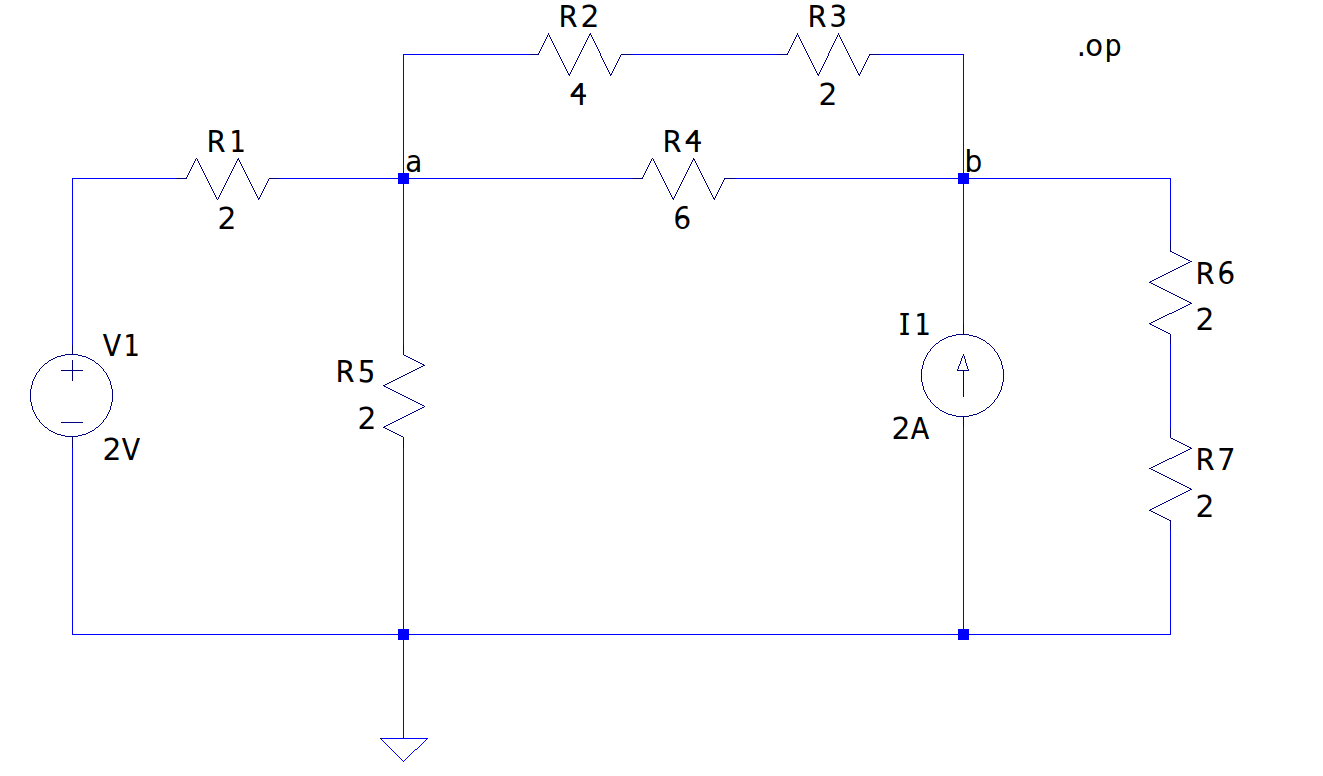
\includegraphics[scale=0.5]{../pictures/circuit.png} % Pas utiliser width=\textwidth pcq il prend la taille de \section{} comme ref
        \caption{Schéma du circuit}
    \end{figure}

    \begin{figure}[H]
        \centering
        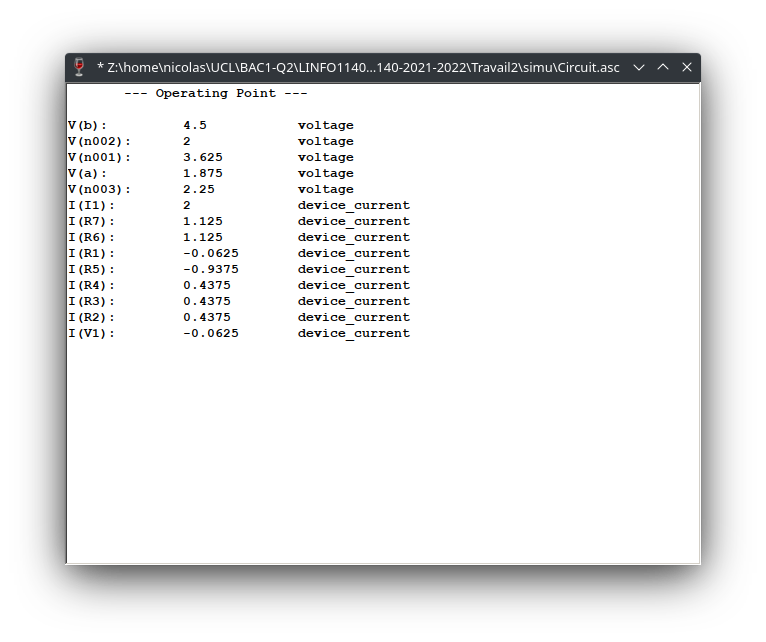
\includegraphics[scale=0.5]{../pictures/resultat.png} % Pas utiliser width=\textwidth pcq il prend la taille de \section{} comme ref
        \caption{Résultat du circuit}
    \end{figure}




    \section{Méthode des noeuds}
    \subsection{Simplification du circuit}
        \subparagraph{}Afin de simplifier les calculs, nous pouvons poser des résistances équivalentes :
            \begin{align*}
                R_{eq_{1}}&=\; (R_2 + R_3)\;//\;R_4 \\
                R_{eq_{1}}&=\; \frac{(R_2 + R_3) \cdot R_4}{(R_2 + R_3) + R_4} \\
                R_{eq_{1}}&=\; \frac{(4 + 2) \cdot 6}{(4 + 2) + 6} \\
                R_{eq_{1}}&=\; \frac{36}{12} \\
                R_{eq_{1}}&=\; 3\;\Omega
            \end{align*}
            
            \begin{align*}
                R_{eq_{2}}&=\; R_6 + R_7 \\
                R_{eq_{2}}&=\; 2 + 2 \\
                R_{eq_{2}}&=\; 4\;\Omega
            \end{align*}
            
        \subparagraph{}On obtient donc le circuit simplifié suivant :
        
            \begin{figure}[H]
                \centering
                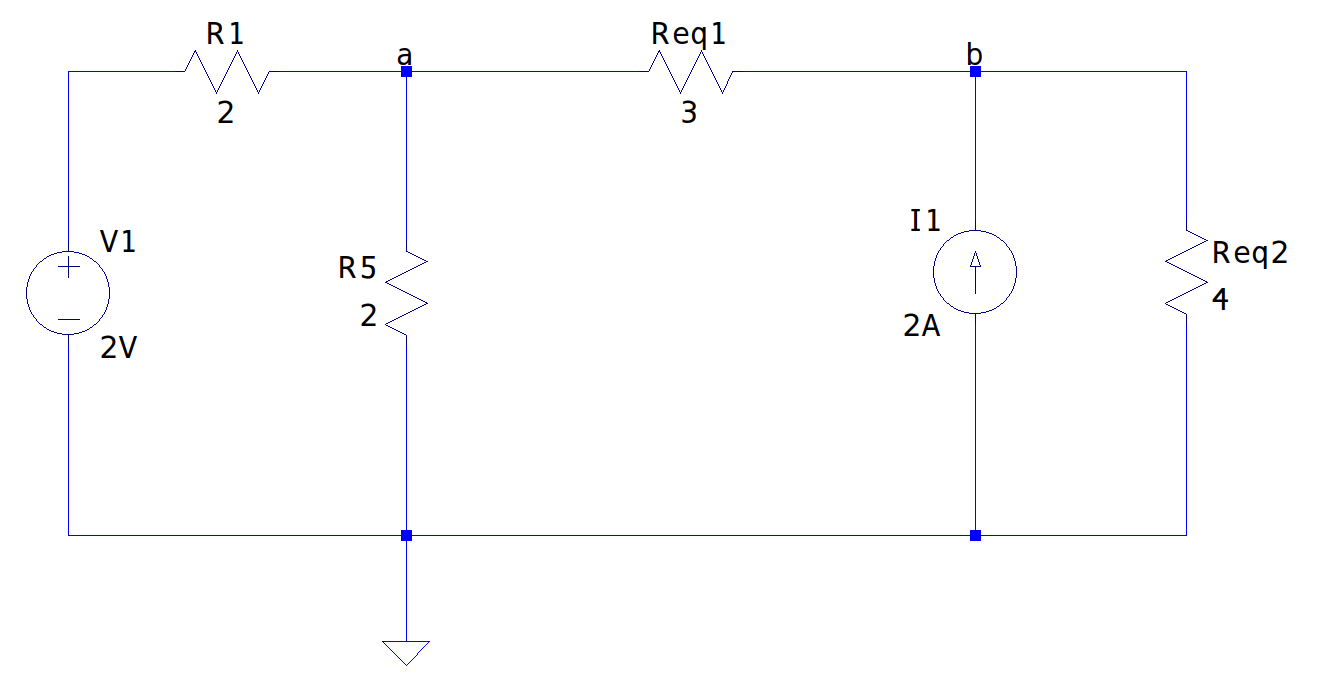
\includegraphics[scale=0.4]{../pictures/simplifie.png}
                \caption{Circuit simplifié}
                \label{fig:simp}
            \end{figure}
    
    \subsection{Sens des courants et tensions}
        \subparagraph{}Ensuite, on définit arbitrairement le sens des courants dans le circuit et puis le sens des tensions de manière opposé au sens des courants :
                \begin{figure}[H]
                    \centering
                    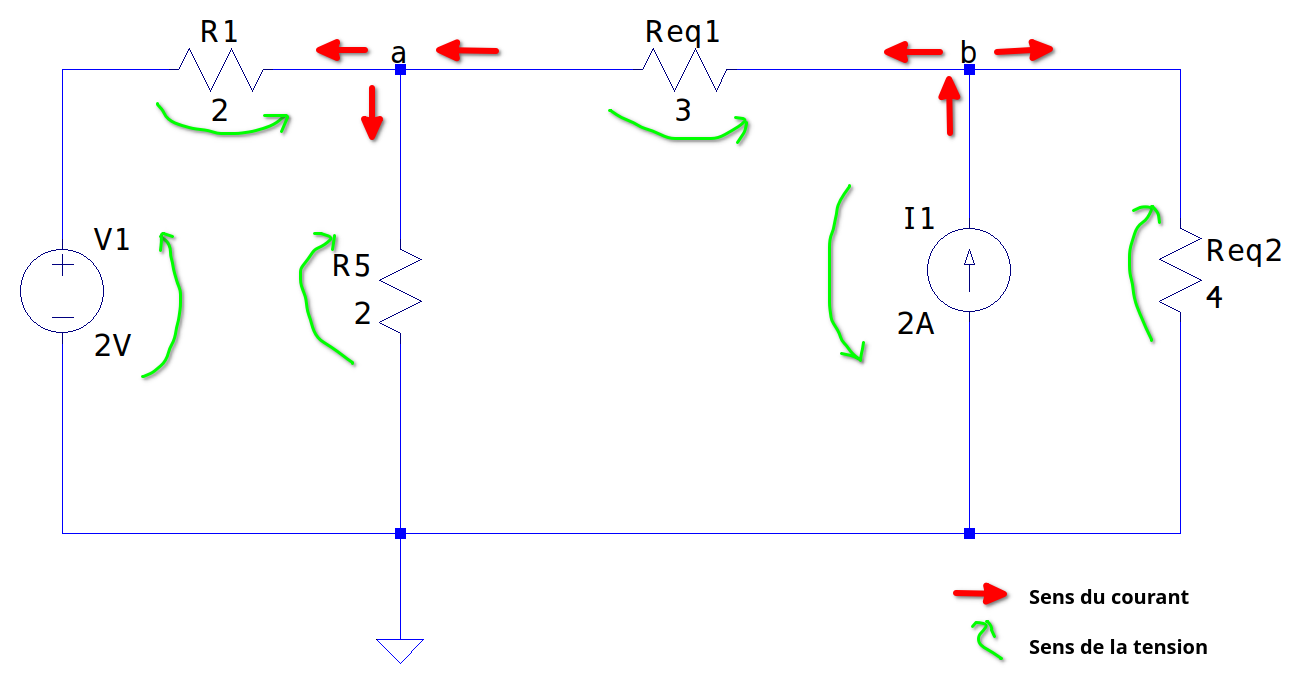
\includegraphics[scale=0.4]{../pictures/sens.png}
                    \caption{Circuit avec le sens des courants en rouge et ceux des tensions en vert}
                    \label{fig:sens}
                \end{figure}
                
                
    \subsection{Écriture des équations}
    \subparagraph{}On cherche la tension aux bornes de a ($V_a$) et la tension aux bornes de b ($V_b$). On sait que l'on peut trouver l'intensité des courants par la formule $I\;=\;\frac{V}{R}$. On sait également grâce à la loi de Kirchhoff que la somme des courants est égale à la somme des courants sortants. On peut donc poser le système suivant :
        \begin{equation*}
            \left \{
               \begin{array}{r c l}
                  \frac{V_b\;-\;V_a}{3} & = \frac{V_a\;-\;2}{2} + \frac{V_a}{2} \\
                  2 & = \frac{V_b}{4} + \frac{V_b\;-\;V_a}{3}
               \end{array}
           \right .
        \end{equation*}
        
    \subsection{Résolution du système d'équation}
    
        \subparagraph{}Pour plus de lisibilité, posons $x = V_a$, $y = V_b$ :
            
            \begin{equation*}
            \left \{
               \begin{array}{r c l}
                  \frac{y\;-\;x}{3} & = \frac{x\;-\;2}{2} + \frac{x}{2} \\
                  2 & = \frac{y}{4} + \frac{y\;-\;x}{3}
               \end{array}
           \right .
        \end{equation*}
        
        \subparagraph{}Supprimons les dénominateurs : 
            \begin{equation*}
                \left \{
                   \begin{array}{r c l}
                      2 \cdot (y\;-\;x) & = 3 \cdot (x\;-\;2) + 3x \\
                      24 & = 3y + 4 \cdot (y\;-\;x)
                   \end{array}
               \right .
            \end{equation*}
        
        \begin{equation*}
            \Rightarrow \left \{
               \begin{array}{r c l}
                  -8x + 2y & = -6 \\
                  -4x + 7y & = 24
               \end{array}
           \right .
        \end{equation*}
        
        \subsubsection{Résolution par l'élimination de Gauss-Jordan}
        
            \[A=\left(
             \begin{array}{cc|c}
                -8 & 2 & -6\\
                -4 & 7 & 24\\
             \end{array}\right)
            \]
            
            \[\Leftrightarrow^{L_1^{(-2)}} \left(
             \begin{array}{cc|c}
                -4 & 1 & -3\\
                -4 & 7 & 24\\
             \end{array}\right)
            \]
            
            \[\Leftrightarrow^{L_{21}^{(-7)}} \left(
             \begin{array}{cc|c}
                -4 & 1 & -3\\
                24 & 0 & 45\\
             \end{array}\right)
            \]
            
            \[\Leftrightarrow^{L_2^{(\frac{1}{24})}} \left(
             \begin{array}{cc|c}
                -4 & 1 & -3\\
                 1 & 0 & 45/24\\
             \end{array}\right)
            \]
            
            \[\Leftrightarrow^{L_{12}^{(4)}} \left(
             \begin{array}{cc|c}
                 0 & 1 & 9/2\\
                 1 & 0 & 15/8\\
             \end{array}\right)
            \]
            
            \[\Leftrightarrow^{L_{12}} \left(
             \begin{array}{cc|c}
                 1 & 0 & 15/8\\
                 0 & 1 & 9/2\\
             \end{array}\right)
            \]
            
            \subparagraph{}On obtient donc :
                \begin{equation*}
                    \left \{
                        \begin{array}{r c l}
                            x & = \frac{15}{8} \\
                            y & = \frac{9}{2}
                        \end{array}
                    \right .
                \end{equation*}
                
            \subparagraph{} On peut donc maintenant calculer $V_a$ et $V_b$ :
            
                \begin{align*}
                    V_a\;&\;=\;x \\
                    V_a\;&\;=\;\frac{15}{8} \\
                    V_a\;&\;=\;1.875\;V \\
                \end{align*}
                
                \begin{align*}
                    V_b\;&\;=\;y \\
                    V_b\;&\;=\;\frac{9}{2} \\
                    V_b\;&\;=\;4.5\;V \\
                \end{align*}

\section{Conclusion}

    \paragraph{}Pour conclure ce travail, je peux affirmer que les résultats sont accord avec la simulation du circuit
    faite sur \textit{LTspice}. Ce travail permet de bien s'imprégner de la méthode des noeuds.


